\subsubsection{Sensoren}
\begin{figure}[h]
\centering
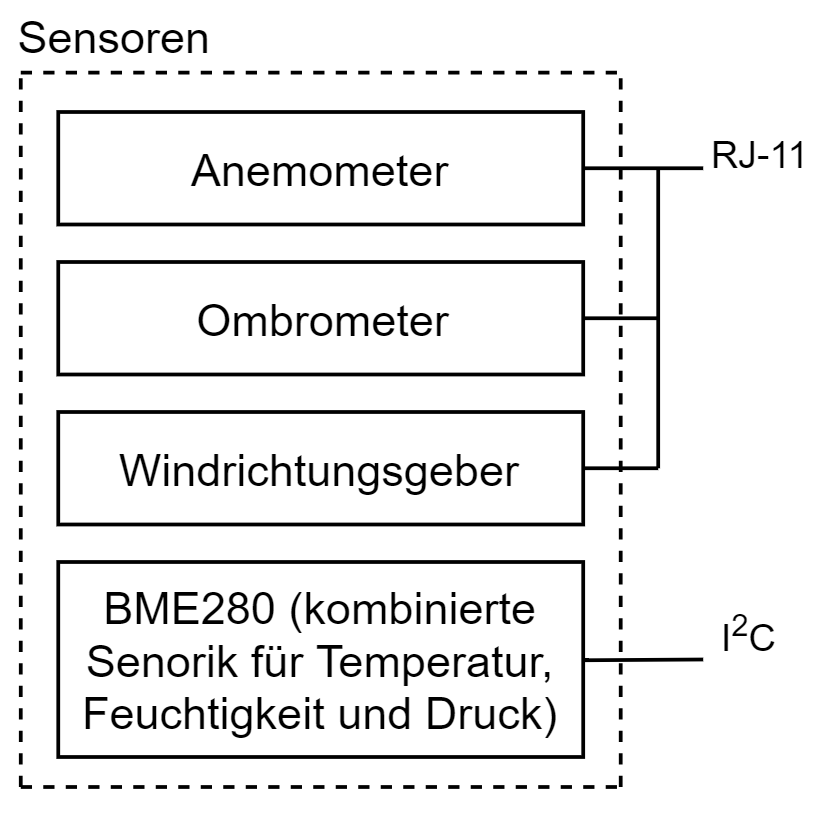
\includegraphics[width=0.5\textwidth]{graphics/Konzeptdiagramme/Sensoren.PNG} 
\caption{Sensoren}
\label{fig:sensoren}
\end{figure}
In dem Block \textit{Sensoren} werden alle Messeinheiten untergebracht. Die Idee dieses Blockes besteht darin, dass dieser adaptiv ist und somit leicht erweitert werden kann (Abbildung \ref{fig:sensoren}).\\
\todo[inline]{Inwiefern kann die Sensorik erweitert werden? Implementieren wir mehr Anschlüsse als gebraucht oder ist bloss die MCU erweiterbar mit einem zusätzlichen Print (aufsteckbar o.ä.)? -Erweiterungsmöglichkeit aufzeigen-}

\subparagraph{Windstärke:}
Die Windstärke wird über ein Schalenanemometer ermittelt. Mittels Reed-Kontakt wird die Drehfrequenz bestimmt und daraus eine Windstärkenstufe nach der Beaufort-Skala zugeordnet.\\
\subparagraph{Windrichtung:}
Die Windrichtung wird mit einer Windfahne gemessen, dessen Position mittels Reed-Kontakten ermittelt werden kann.\\
\subparagraph{Lufttemperatur, -Feuchtigkeit $\&$ -Druck:}
Die Lufttemperatur, Luftfeuchtigkeit und der Luftdruck werden über ein IC-Bauteil gemessen.\\
\todo[inline]{vellicht bitz detailierter?}
\subparagraph{Regenmenge:}
Für die Bestimmung der Regenmenge wurde auf eine alte aber effiziente Methode zurückgegriffen, das Kipplöffelprinzip. Bei diesem Prinzip füllt das Regenwasser einen Löffel der sich in der Ausgangsposition befindet, dieser Löffel kippt bei einer gewissen Menge und lässt einen zweiten Löffel in die Ausgangsposition heben. Über einen Reed-Kontakt wird die Kippfrequenz bestimmt, und daraus kann auf die Regenmenge zurück geschlossen werden.\\
\subparagraph{Sonnenstunden:}
Um die Sonnenstunden zu ermitteln, wird ein Sensor verwendet welcher die Bestrahlungsstärke misst. Die Sonnenstunden werden errechnet, wobei die Solarkonstante eine wichtige Rolle spielen dürfte.\\
\newpage